\documentclass[portuguese]{textolivre}

% metadata
\journalname{Texto Livre}
\thevolume{18}
%\thenumber{1} % old template
\theyear{2025}
\receiveddate{\DTMdisplaydate{2024}{10}{18}{-1}}
\accepteddate{\DTMdisplaydate{2024}{11}{19}{-1}}
\publisheddate{\today}
\corrauthor{Jackson Wilke da Cruz Souza}
\articledoi{10.1590/1983-3652.2025.55346}
%\articleid{NNNN} % if the article ID is not the last 5 numbers of its DOI, provide it using \articleid{} commmand 
% list of available sesscions in the journal: articles, dossier, reports, essays, reviews, interviews, editorial
\articlesessionname{articles}
\runningauthor{Souza, Semcovici e Pardo}
%\editorname{Leonardo Araújo} % old template
\sectioneditorname{Daniervelin Pereira}
\layouteditorname{João Mesquita}

\title{Proposta de algoritmo de classificação automática de papéis semânticos em português no âmbito do modelo Abstract Meaning Representation}
\othertitle{Proposal of an algorithm for automatic classification of semantic roles in Portuguese within the Abstract Meaning Representation model}

\author[1]{Jackson Wilke da Cruz Souza~\orcid{0000-0003-1881-6780}\thanks{Email: \href{mailto:jackcruzsouza@gmail.com}{jackcruzsouza@gmail.com}}}
\author[2]{Pedro Semcovici~\orcid{0009-0008-8455-8509 }\thanks{Email: \href{mailto:pedrosemcovici@usp.br}{pedrosemcovici@usp.br}}}
\author[2]{Thiago Alexandre Salgueiro Pardo~\orcid{0000-0003-2111-1319 }\thanks{Email: \href{mailto:taspardo@icmc.usp.br}{taspardo@icmc.usp.br}}}
\affil[1]{Universidade Federal da Bahia,Instituto de Ciência, Tecnologia e Inovação, Camaçari, BA, Brasil.}
\affil[2]{Universidade de São Paulo, Escola de Artes, Ciências e Humanidades, São Paulo, SP, Brasil.}

%\usepackage{calc,easyReview,enumitem,longtable,multirow,tabularx,ulem}
%\newcolumntype{Y}{>{\centering\arraybackslash\hsize=1\hsize}X}%Custom-made column type to ensure that the columns are of equal width and center-aligned
%\usepackage{enumitem,colortbl,multirow,longtable}
\usepackage{multirow}

\addbibresource{article.bib}

\begin{document}
\maketitle
\begin{polyabstract}
\begin{abstract}
  O nível semântico em Processamento de Linguagem Natural (PLN) apresenta desafios significativos devido à complexidade dos fenômenos, que são menos suscetíveis a descrições objetivas. Nem todas as abordagens linguísticas, como o modelo teórico de papéis semânticos proposto por \textcite{cançado2017}, são facilmente implementáveis em sistemas computacionais devido à sua variabilidade terminológica e metodológica. O modelo Abstract Meaning Representation (AMR) \cite{banarescu2013,weischedel2013} tem se destacado por oferecer uma representação clara da estrutura argumental, proporcionando explicabilidade tanto para humanos quanto para sistemas computacionais sobre como o sentido se organiza em sentenças de línguas naturais. Baseando-se no AMR, desenvolvemos um classificador automático de papéis semânticos. Utilizando técnicas de Aprendizado de Máquina, nosso classificador foi treinado e testado em um corpus multigênero em Português do Brasil. Realizamos dois experimentos: o primeiro comparando Argumentos 0 e 1, e o segundo comparando Argumentos de 0 a 4, obtendo melhores resultados no primeiro experimento. Os resultados ressaltam a importância da aplicação de modelos semânticos em PLN para o português e abrem possibilidades para novas iniciativas de pesquisas.

  
  

\keywords{Papéis semânticos \sep Abstract Meaning Representation \sep Processamento de Linguagem Natural}
\end{abstract}

\begin{english}
\begin{abstract}
  Semantic level in Natural Language Processing (NLP) presents significant challenges due to the phenomena’s complexity, which are less amenable to objective description. Not all linguistic approaches, such as the semantic role theory proposed by \textcite{cançado2017}, can be easily implemented in computational systems due to their terminological and methodological variability. The Abstract Meaning Representation (AMR) model \cite{banarescu2013,weischedel2013} has gained prominence for providing a clear representation of argument structure, offering explicability both for humans and computational systems on how meaning is organized in sentences of natural languages. Based on AMR, we developed an automatic semantic role classifier. Using Machine Learning techniques, our classifier was trained and tested on a multi-genre corpus in Brazilian Portuguese. We conducted two experiments: the first comparing Arguments 0 and 1, and the second comparing Arguments 0 to 4, achieving better results in the former. The results highlight the importance of applying semantic models in NLP for Portuguese and open possibilities for new research initiatives.
  
  
\keywords{Semantic roles \sep Abstract Meaning Representation \sep Natural Language Processing}  

\end{abstract}
\end{english}
\end{polyabstract}

\section{Introdução}\label{sec-intro}

O processo de escrita é uma das atividades mais complexas que o ser
humano é capaz de realizar, em razão de vários fatores, a exemplo das
exigências feitas à memória e ao raciocínio durante o momento de
produção \cite{garcez2020}. São inúmeros os conhecimentos e habilidades que
precisam ser articulados e harmonizados para que o texto tome forma.
Tendo em vista esse seu caráter complexo, ainda são recorrentes falsas
crenças sobre a produção textual, que levam pessoas a acreditarem que
podem dominá-la a partir de ``dicas'' desvinculadas de seu contexto de
produção.

A ideia de que fórmulas pré-fabricadas e ``dicas'' isoladas são métodos
cabíveis no ensino de produção textual, apenas negligencia as etapas
necessárias que caracterizam um texto adequado conforme seu contexto de
produção \cite{garcez2020}. O processo de escrita é uma atividade que
carece de idas e vindas, pois deve admitir três grandes momentos que se
intercalam e devem ser compreendidos de modo indissociável: o do
planejamento, o da escrita propriamente dita e o da revisão \cite{antunes2005}. Enquadrar esse processo em uma perspectiva prescrita e linear
pode resultar em estudantes frustrados pela construção de textos
truncados e artificiais.

Essa realidade se agrava quando observamos o cenário acadêmico, em que
as exigências com relação a produções textuais se intensificam. As
expectativas quanto a essas produções não se limitam à utilização
adequada da norma-padrão ou a vocabulários específicos; expandem-se para
aspectos implícitos de produção que precisam ser considerados, como o
que pode ser dito, por quem, de que forma, sob que ponto de vista e
fundamentado em qual autor \cite{oliveira2024}.

Pensando na comunidade discursiva acadêmica, uma das produções textuais
mais demandadas em cursos de graduação da área de humanas é o artigo
acadêmico \cite{motta-roth2010}. Por ser um dos principais
veículos de divulgação científica, a circulação desse gênero na academia
é incontornável, sendo bastante exigido o seu consumo e produção por
parte de professores, estudantes e pesquisadores. Embora seja uma
produção essencialmente ligada ao meio universitário, sua feitura é
quase sempre exigida sem antes ser ensinada. Esse fato pode levar os
alunos a somarem suas dificuldades com o processo de escrita à
dificuldade de produzir um texto do qual desconhecem seu contexto de
produção, estrutura composicional e outras ``dimensões escondidas''
\cite{street2010} que perpassam a construção de um artigo.

Ao exigir do autor capacidade de síntese, descrição, análise e
argumentação, utilizando-se das convenções próprias à determinada área,
o artigo contempla informações geradas em pesquisas a serem submetidas a
apreciações públicas \cite{motta-roth2010}. Sua relevância remonta
à popularização da ciência que, por sua vez, possui a potencialidade de
descrever fenômenos sociais e até mesmo gerar algum impacto benéfico ao
público em geral.

A partir dessas pontuações, torna-se clara a importância de produzir
artigos acadêmicos e a responsabilidade do seu produtor de popularizar
os conhecimentos produzidos na esfera acadêmica. Quando essa tarefa de
produção precisa ser desenvolvida por graduandos e estes normalmente não
recebem orientação para tal, muitas vezes, recorrem a materiais digitais
sobre esse assunto, pois lhes propiciam as mais variadas estratégias de
ensino de acordo com o ritmo e as preferências do estudante \cite{falkembach2005}. Um fator que pode justificar essa recorrência é a facilidade de
acesso a plataformas digitais, que disponibilizam, na maioria das vezes
de forma gratuita, conteúdos digitais educacionais. Antigamente, os
estudantes consultavam manuais impressos que ensinavam a como produzir
textos acadêmicos, hoje, frente aos recursos tecnológicos, os locais de
aprendizagem se ampliam para a cibercultura. Como cibercultura,
compreendem-se vários ambientes da esfera digital que abrigam
informações, até mesmo os que simulam uma sala de aula a partir de
vídeos \cite{martins2018,rocha2005}.

Tendo a cibercultura se tornado uma potencializadora de novas abordagens
educativas, deve-se averiguar sua eficiência enquanto ferramenta de
ensino, a forma como se ensina determinados conteúdos, a exemplo da
produção textual de artigo acadêmico e seus aspectos constitutivos, foco
do presente estudo. Nesse sentido, traçamos dois objetivos para este
trabalho: identificar e analisar objetos de ensino explorados em
videoaulas sobre artigo acadêmico publicadas na plataforma YouTube.

Para tanto, organizamos este artigo em 5 seções, a saber: esta
introdução, contendo uma contextualização inicial sobre o objeto de
investigação da pesquisa, a problemática que o envolve e os objetivos
delineados; o embasamento teórico, no qual apresentamos os pressupostos
que fundamentam o estudo --- as práticas de ensino de Língua Portuguesa
em contexto didático-digital \cite{laurentino2023}, o artigo
acadêmico \cite{motta-roth2010}, as etapas de produção textual
(Antunes, 2003) e os objetos de ensino \cite{linodearaujo2014}; a
metodologia, na qual explicitamos a abordagem e o tipo de pesquisa, bem
como os procedimentos de coleta e análise de dados; os resultados,
contendo a exploração dos objetos de ensino contemplados nas videoaulas
sobre ensino de produção de artigo acadêmico; as considerações finais,
nas quais sinalizamos algumas implicações advindas dos resultados
alcançados.
\section{Revisão da literatura}\label{sec-revisão}

Nesta seção, serão apresentados trabalhos recuperados da literatura que
dialogam direta ou indiretamente com a temática desenvolvida nesta
pesquisa, sobretudo relacionados aos papéis semânticos em PLN e à
aplicação de SRL.

\subsection{Papéis semânticos nos estudos de PLN}\label{sub-sec-papeissemanticos}

Segundo \textcite{banarescu2013}, o modelo AMR objetiva capturar e
representar explicitamente aspectos do significado de uma sentença. Esse
modelo teórico propõe a enumeração de argumentos na tentativa de
simplificar a proposta de papéis semânticos. \textcite{weischedel2013} apontam que na AMR, tradicionalmente, segue-se a seguinte
proposta:

\begin{itemize}
\item[Arg0]\label{arg0}: refere-se ao argumento da ação que desempenha o papel de agente;
\item[Arg1]\label{arg1}: refere-se ao argumento principal que é afetado pela ação
  expressa pelo verbo, correspondendo, em geral, ao objeto direto;
\item[Arg2]\label{arg2}: refere-se a um argumento secundário ou ao objeto indireto em
  construções que apresentam verbos;
\item[Arg3, Arg4 e Arg5]\label{arg345}: são termos menos frequentes nas construções
  linguísticas, ocorrendo em construções verbais mais complexas, como
  para o verbo ``dar'' ou ``entregar''.
\end{itemize}

A partir dessas definições, é importante ressaltar que a proposta do
modelo AMR pode ou não levar em conta aspectos morfossintáticos e/ou a
ordem em que os itens lexicais ocorrem nas sentenças. O Arg0, por
exemplo, é definido apenas a partir de aspectos semânticos; todos os
outros argumentos levam em conta, em alguma medida, informações
gramaticais que consideram a ordem e/ou a classificação morfossintática.
Outro ponto importante desse modelo é que itens lexicais/\emph{tokens}
que não contribuem fortemente para a construção dos sentidos em
determinadas sentenças (como determinantes/artigos) não são considerados
na análise, dando-se ênfase na estrutura argumental.

A título de exemplificação, tem-se a sentença apresentada em \ref{itm3}, que
foi extraída do \emph{corpus} AMR-PT \cite{inacio2023}, que
contempla sentenças extraídas da obra ``O pequeno príncipe'', dentre
outros gêneros textuais, atualmente.

\begin{enumerate}[start=3,label={(\arabic{enumi})}]
    \item\label{itm3} Meu desenho não representava um chapéu.
\end{enumerate}

De acordo com a proposta AMR, na sentença exemplificada em \ref{itm3}, tem-se
dois argumentos: ``desenho'' é o argumento principal em relação ao verbo
``representar'' e, por isso, recebe a classificação de Arg1; e
``chapéu'', que desempenha o papel de ``objeto'', recebe a classificação
Arg2. Os itens lexicais ``meu'' e ``não'' indicam, respectivamente, a
relação de posse e a polaridade negativa da sentença. Tais relações
também são consideradas e representadas no modelo AMR. Por fim, o item
``um'' não faz parte da estrutura argumental pois não exerce modificação
significativa sobre ``chapéu'', ainda que desempenhe função de
indeterminação sobre ele.

Além disso, o modelo propõe possibilidades de representação do
conhecimento semântico, aspecto extremamente importante para
implementação computacional. Uma dessas representações é a
\emph{estrutura de grafos}, em que os nós representam eventos e
entidades mencionados na sentença; já as arestas representam as relações
entre os nós. A \Cref{fig-01} representa a estrutura argumental do exemplo em \ref{itm3}.

\begin{figure}[htpb]
  \centering    
  \begin{minipage}{.75\textwidth}
  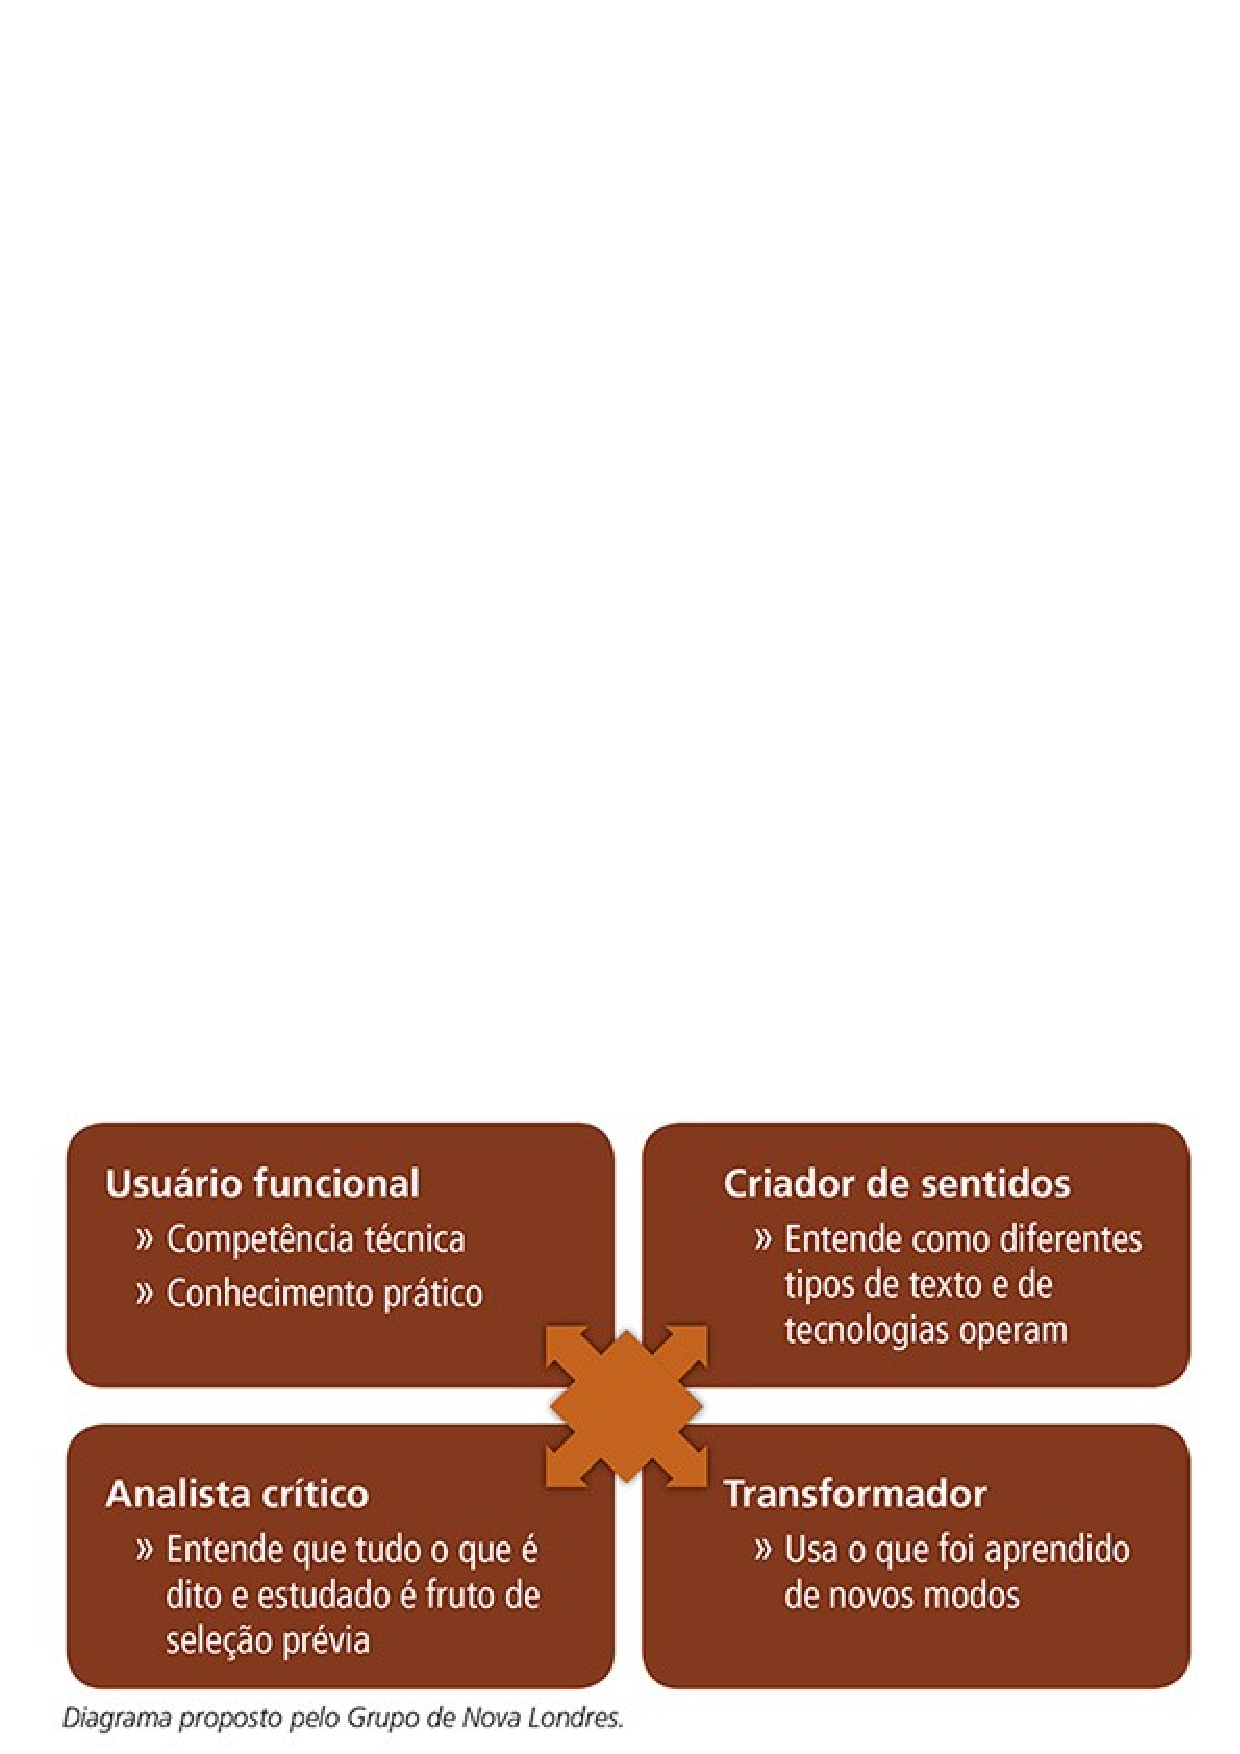
\includegraphics[width=\textwidth]{figure01.png}
  \caption{Exemplo de grafo AMR.}
  \label{fig-01}
  \source{Adaptado de \textcite{anchiêta2022}.}
  \end{minipage}
\end{figure}

Outra possibilidade de representação é por meio de \emph{notação lógica}
(\Cref{fig-02}), em que, a partir da identificação léxica do predicado,
apontam-se os tipos de argumentos, seus respectivos itens lexicais e a
relação semântica estabelecida entre eles. Por fim, na \emph{notação
Penman} (\Cref{fig-03}), feita em formato textual, há delimitação de
instâncias, que são os itens lexicais que funcionam como argumentos e/ou
predicados nas sentenças, a estrutura argumental entre as instâncias e
as relações que podem estabelecer entre si. Cabe destacar que as três
figuras equivalem à mesma representação semântica, sendo que a \Cref{fig-01},
por seu apelo gráfico, pode ser melhor interpretável por humanos, ao
passo que as Figuras 2 e 3 permitem implementações computacionais por
serem notações lógicas.

\begin{figure}[htpb]
\begin{minipage}{.45\textwidth}
  \centering
  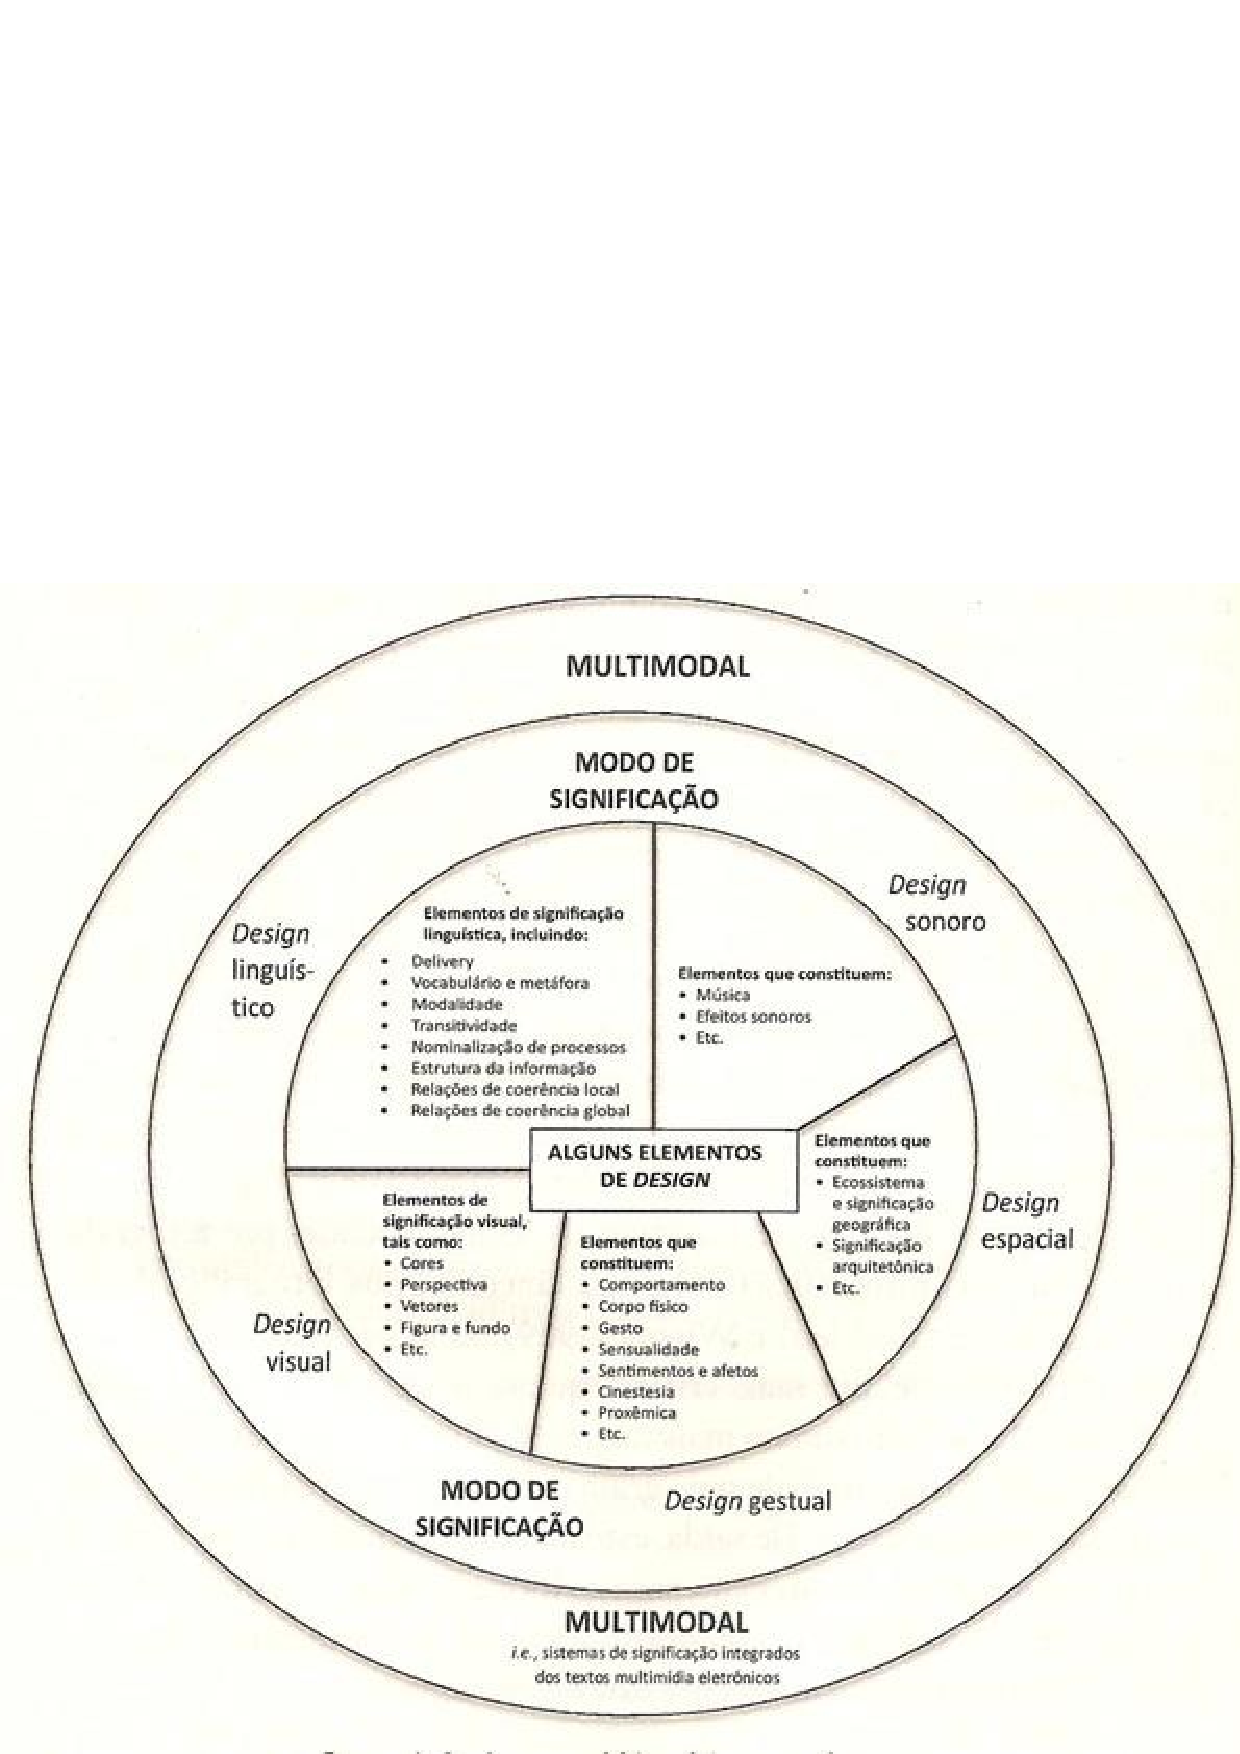
\includegraphics[width=\textwidth]{figure02.jpg}
  \caption{Exemplo de notação lógica no modelo AMR.}
  \label{fig-02}
  \source{Elaborado pelos autores.}
\end{minipage}%
\hfill
\begin{minipage}{.45\textwidth}
  \centering
 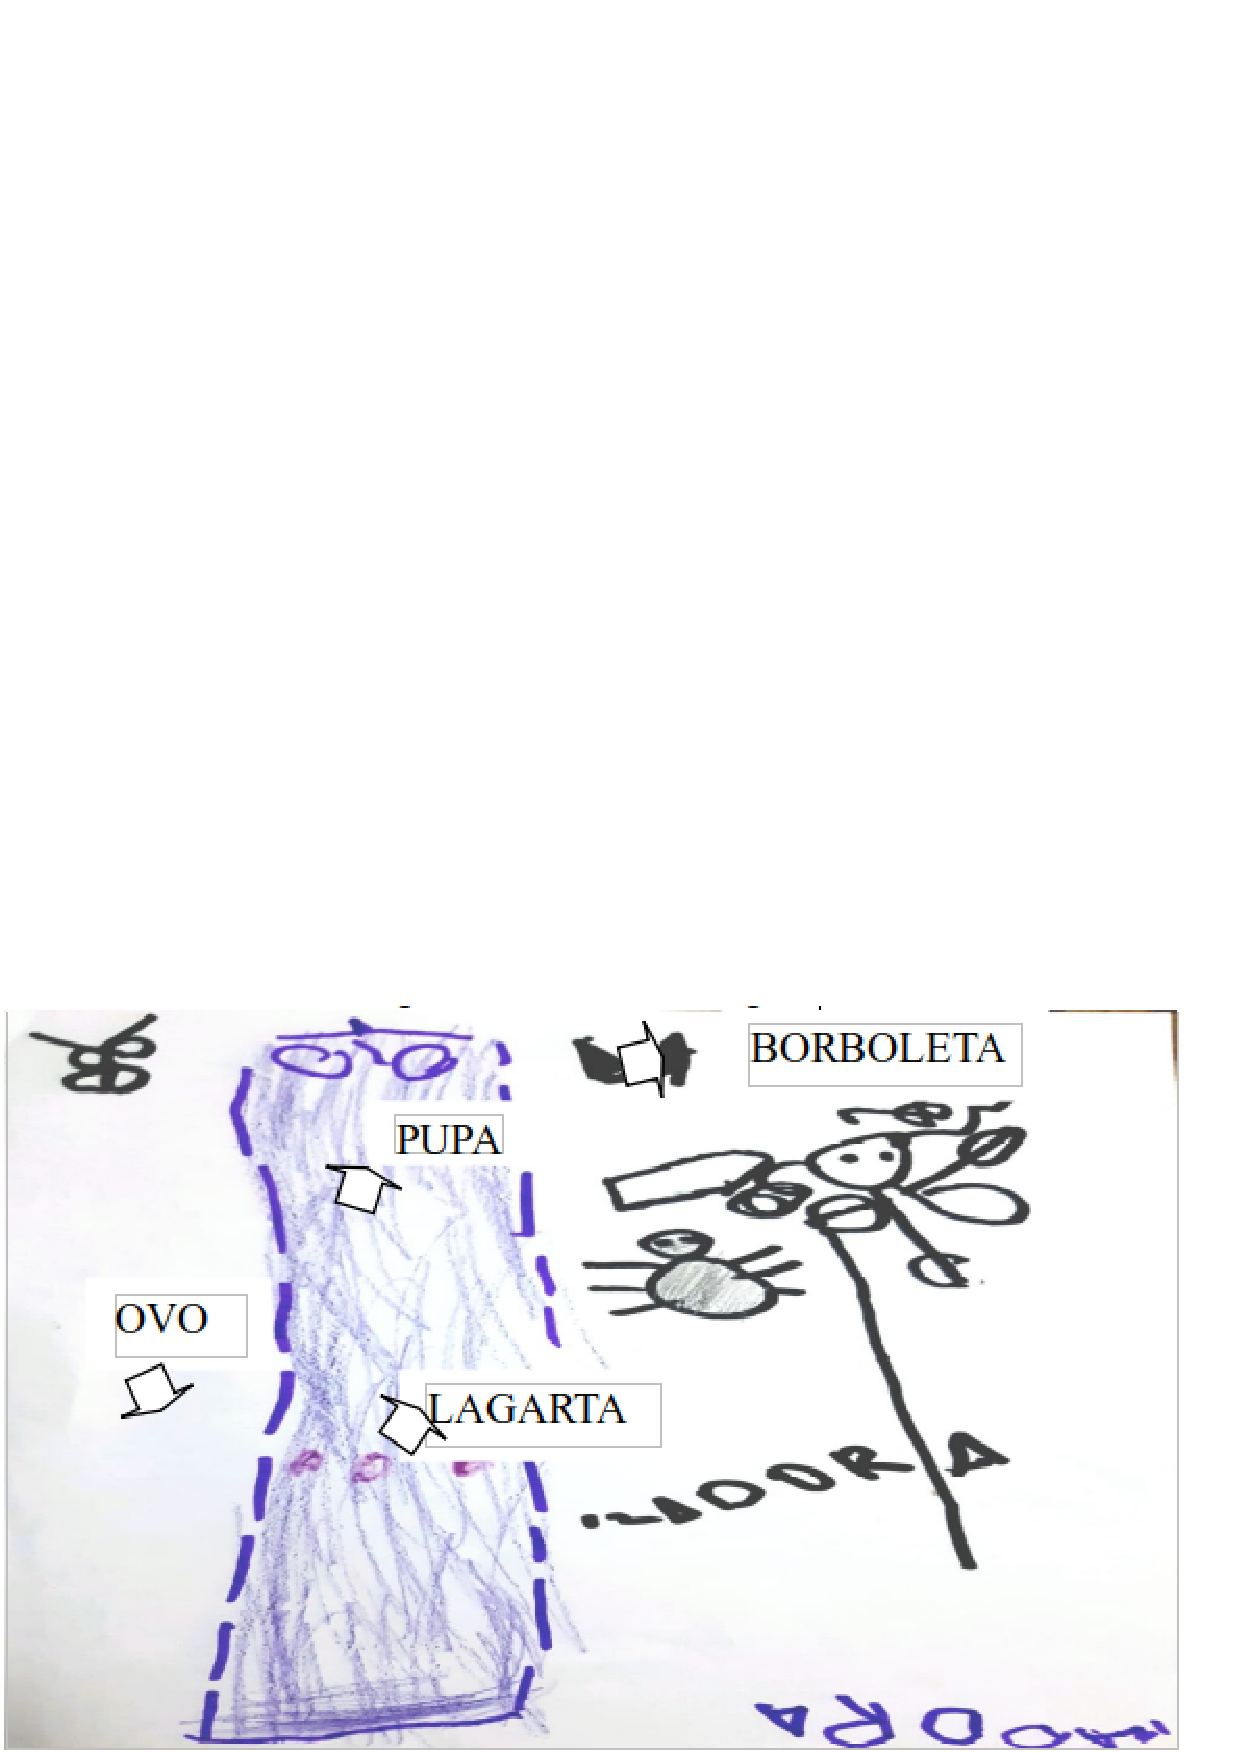
\includegraphics[width=\textwidth]{figure03.jpg}
  \caption{Exemplo de notação Penman no modelo AMR.}
  \label{fig-03}
  \source{Elaborado pelos autores.}
\end{minipage}
\end{figure}

Outro aspecto importante na proposta do modelo é a classificação dos
conceitos. De acordo com \textcite{anchiêta2022}, os conceitos AMR podem
ser classificados em \emph{concretos} (palavras em suas formas
lexicalizadas, como ``mulher'' e ``homem''), \emph{framesets} do
\emph{Proposition Bank} -- PropBank\footnote{PropBank pode ser definido
  como um recurso de sentenças anotadas com funções semânticas
  \cite{jurafsky2023}. Por conta da dificuldade de se obter um
  conjunto ``universal'' de papéis semânticos, como demonstrados nesta
  seção, nos PropBanks convencionou-se que as relações semânticas são
  numeradas (ao invés do uso de seus nomes), que é justamente a
  filosofia adotada pela AMR.} -- \cite{palmer2005} ou
\emph{abstratos} (que não correspondem a nenhuma unidade lexical das sentenças, como ``\%'' e ``endereço de e-mail'', por exemplo).

\subsection{Trabalhos relacionados à SRL}\label{sub-sec-trabalhos}

De acordo com \textcite{hartmann2017}, SRL é uma tarefa em PLN
que detecta eventos descritos em sentenças e os participantes desses
eventos. Os eventos ocorrem nas sentenças sob formas morfológicas de
verbos, nomes, adjetivos e advérbios; porém, a classe que mais é
explorada na literatura é a dos verbos, pois expressam eventos, além de
ser impossível construir orações completas com ausência de verbos. As
demais classes de palavras não expressam eventos da mesma forma que os
verbos, nem em proporção.

Ainda segundo \textcite{hartmann2017}, os métodos empregados na
anotação automática de papéis semânticos são, na maioria, com base em
AM. Nesse contexto, é necessário que haja \emph{corpora} linguísticos
anotados para que os algoritmos de AM possam ser treinados e avaliados
quanto ao desempenho da tarefa a que eles foram submetidos. A literatura
aponta alguns \emph{corpora} disponíveis com anotação AMR, importantes
para as tarefas de SRL, a saber: \textcite{xue2014} para o inglês;
\textcite{vanderwende2015} com uma abordagem multilíngue para
Francês, Alemão, Espanhol e Japonês; \textcite{damonte2019} %\alert{Damonte e Cohen (2018)} 
para as línguas italiana, espanhola, alemã e chinesa; \textcite{migueles2018} especificamente para o espanhol; e \textcite{anchiêta2018} e
\textcite{inacio2023}, para o PB. Destaca-se que há também
recursos com papéis semânticos desvinculados da estruturação completa
proposta pela AMR, como é o caso do PropBank do inglês, citado
anteriormente, e o PropBank.Br \cite{duran2012} e o recente PBP
(\emph{Porttinari-base Propbank}) para o português \cite{freitas2024}.

Em especial, o \emph{corpus} para o PB é composto por sentenças anotadas
com o modelo AMR para diferentes gêneros textuais. A primeira versão do
\emph{corpus} apresentava sentenças extraídas do romance ``O pequeno
príncipe'', tido como \emph{corpus} ``\emph{little prince}''. Em sua
segunda versão, o escopo de domínio foi ampliado para notícias extraídas
do jornal Folha de S. Paulo \cite{duran2012}, tido como o
\emph{corpus} ``\emph{news}''. Em sua versão mais recente\footnote{Disponível
  em: \href{https://github.com/nilc-nlp/AMR-BP}{GitHub -
  nilc-nlp/AMR-BP}. Acesso em: 20 jul.2024.}, o AMR-PB apresenta textos
opinativos, tido como \emph{corpus} ``\emph{opisums}'', e científicos,
tido como \emph{corpus} ``\emph{sci}''. Ademais, todos os \emph{corpora}
apresentam sentenças anotadas, identificando os papéis semânticos
seguindo a metodologia do PropBank.Br \cite{duran2012}.

Com relação ao PropBank.Br, \textcite{duran2012} destacam que o
\emph{corpus} é um repositório de proposições, alinhando-se ao que
\textcite{fillmore1968} apresenta sobre a estrutura base de uma frase, a saber:
um conjunto de relações entre substantivos e verbos, sem modificadores
de tempo, negação, aspecto e modo. Segundo as autoras, os verbos recebem
um código que indica seu sentido com relação ao \emph{frame} em que a
sentença está associada; já os argumentos são anotados com rótulos de
função numerados (de Arg0 a Arg5) e os modificadores são anotados com
rótulos de função ArgMs (Modificadores de argumento).

Vale a pena ressaltar que os \emph{corpora} delimitados aqui seguem as
diretrizes da literatura quanto ao PLN. Os conjuntos de dados
linguísticos acompanham os apontamentos de \textcite{gildea2002}, já
que representam semanticamente os papéis temáticos distanciando-se de
detalhamentos analíticos, ao passo que se aproximam da objetividade e
simplificação de rótulos para garantir melhor desempenho no processo de
classificação automática.

Partindo de \emph{corpora} anotados, é possível aplicar diferentes
técnicas de AM. O trabalho de \textcite{hartmann2015} realizou a análise
automática de papéis semânticos utilizando AM nos \emph{subcorpora news}
e \emph{opisums}. Aplicando diferentes abordagens (utilizando ou não
árvores sintáticas treinadas), os autores obtiveram Medida-F de 87,8\%
para o \emph{corpus news}, e 94,5\% para o \emph{corpus opisums}.

Hartmann, \textcite{duran2012} realizaram a avaliação de dois sistemas
de SRL para textos jornalísticos. O sistema desenvolvido por \textcite{fonseca2013} teve o propósito de anotar automaticamente os papéis
semânticos para o PB, sem lançar mão de ferramentas de PLN externas ao
sistema desenvolvido; os resultados dessa avaliação indicam uma Medida-F
de 68\%. Já o sistema de \textcite{alva-manchego2012} empregou a abordagem
supervisionada de AM e obteve Medida-F de 79,6\%. Destaca-se que ambos
os trabalhos foram baseados no \emph{corpus} PropBank.Br.

\textcite{ilmy2021} realizaram a análise de frases em indonésio
utilizando a AMR com abordagem de aprendizado de máquina. Inspirado no
trabalho de \textcite{zhang2019}, o sistema desenvolvido por \textcite{ilmy2021} compreende três etapas: (i) previsão de pares de palavras, (ii)
previsão de rótulos e (iii) construção de grafos. Em (i), utiliza-se um
componente de análise de dependência para obter as conexões entre
palavras. Em (ii), emprega-se um algoritmo de aprendizado supervisionado
para prever os rótulos entre as conexões. Em (iii), a partir dos rótulos
previstos, é criado o grafo da sentença em AMR. Avaliado com uma base de
dados de frases simples coletadas de artigos e notícias, o modelo
atingiu uma pontuação SMATCH\footnote{SMATCH é uma métrica que tem como
  objetivo avaliar estruturas semânticas em ocorrências linguísticas
  \cite{cai2013}.} de 0,820.

% !TeX root = main.tex

\section{Metodología}\label{sec-metodología}

La metodología de la investigación la entendemos como el conjunto de
procedimientos y técnicas que el equipo investigador ha utilizado en el
diseño, desarrollo y análisis del estudio. En este caso concreto, el
método utilizado ha sido de corte mixto, utilizando técnicas
cualitativas y cuantitativas. Las cualitativas se han basado en la
etnografía virtual de los datos generados en los sNOOC y las
conclusiones del juicio del equipo de expertos. Las cuantitativas
provienen de los cuestionarios de satisfacción del alumnado y de los
datos de interacción del alumnado en la plataforma de aprendizaje.


\subsection{Objetivos e hipótesis}\label{sub-sec-objetivosehipotesis}

El objetivo general de este estudio es analizar el proceso de creación
de redes comunicativas de estudiantes para la implementación de sNOOC
como método de evaluación continua en la UAD y su repercusión en la capa
social como modelo de formación mediática en personas de la tercera
edad. Con base en este objetivo general, los objetivos específicos hacen
referencia a:

\begin{itemize}
\item
Objetivo Específico 1 (OE1): Investigar las percepciones y opiniones
de las redes comunicativas de estudiantes respecto a la utilidad y
efectividad de un sNOOC como método de evaluación continua y su
impacto en la motivación hacia el aprendizaje.
\item
Objetivo Específico 2 (OE2): Examinar el proceso de desarrollo de las
redes comunicativas de estudiantes para la creación de contenidos de
los sNOOC, centrándose en el impacto del uso de pedagogías inclusivas,
IA y Metaverso en EAD.
\item
Objetivo Específico 3 (OE3): Evaluar el nivel de implicación activa de
las redes comunicativas de estudiantes en la plataforma de la UNED y
en la creación colaborativa del sNOOC en tmooc.es.
\end{itemize}

A continuación, se formulan las hipótesis para dar respuesta a las
relaciones causales:

\begin{itemize}
\item
Hipótesis 1 (H1-OE1): Si las redes comunicativas de estudiantes
perciben el sNOOC como una herramienta efectiva y útil para la
evaluación continua, aumentará su motivación intrínseca hacia el
aprendizaje y su participación en las actividades y recursos del
itinerario de aprendizaje propuesto.
\item
Hipótesis 2 (H2-0E2): Si el modelo sNOOC es diseñado y aplicado
considerando criterios pedagógicos inclusivos y herramientas
tecnológicas adecuadas, mejorará la comprensión de los contenidos por
parte de las redes comunicativas de estudiantes, incrementando su
satisfacción general con la experiencia de EAD.
\item
Hipótesis 3 (H3-OE3): Si el itinerario de aprendizaje en sNOOC está
basado en pedagogías inclusivas, se incrementará el compromiso activo
de las personas participantes, reflejado en una mayor interacción,
colaboración en equipo y corresponsabilidad en la construcción
colectiva del conocimiento.
\end{itemize}


\subsection{Muestra, instrumentos y análisis de
	datos}\label{sub-sec-muestrainstrumentos}
	
	El objeto de estudio de esta investigación son las interacciones del
	alumnado en la plataforma ALF de la UNED, contando con la participación
	de 79 personas, 57 mujeres y 22 hombres; 1 de nacionalidad croata y, el
	resto, española. Estos participantes han sido estudiantes del Máster
	Universitario en Educación y Comunicación en la Red y, dentro de este,
	de la asignatura ``Escenarios Virtuales para la participación'', una
	disciplina con contenidos relacionados con la educación mediática. En
	este caso concreto, para estructurar el método cuantitativo, se han
	utilizado los cuestionarios con preguntas diseñadas para recopilar datos
	cuantitativos correspondiente al curso 2023/2024.
	
	Referido a la plataforma ``tmooc.es'' donde este grupo de estudiantes
	creó los sNOOC, se ha realizado un análisis de estas propuestas tomando
	también esos entornos como objeto de estudio. Se tuvieron en cuenta los
	registros de datos relacionados con la dedicación en la creación de los
	sNOOC. Los sNOOC seleccionados son los siguientes: ``Introdúcete al
	mundo de Facebook'' (sN1), ``Senior 3.0'' (sN2), ``Correo electrónico
	son misterios: alfabetización digital para personas mayores'' (sN3),
	``Enredados en la edad dorada: dominar Facebook e Instagram con
	confianza'' (sN4), ``Healthy seniors network'' (sN5), ``Estas a un clic
	de conocer el mundo digital'' (sN6), ``Familias y aprendizaje en red''
	(sN7) y ``Google e inteligencia artificial, tus compañeros digitales''
	(sN8). En cuanto al enfoque cualitativo, se consideraron los datos
	generados a través de los sNOOC y las conclusiones del juicio de 22
	personas expertas internacionales, con el fin de validar hipótesis y
	evaluar riesgos o problemáticas presentes en el proyecto formativo. Para
	analizar los datos cuantitativos y cualitativos se utilizaron los
	programas SPSS y Atlas.ti, respectivamente. Estos aspectos se han
	organizado en categorías que se ajustan a las dimensiones de la
	educación inclusiva.

% !TeX root = main.tex


\section{Resultados}\label{sec-resultados}
Los resultados de este estudio se han organizado en torno a dos
categorías fundamentales. En primer lugar, la Categoría 1 hace
referencia a ``Acceso, equidad y participación''; y, en segundo lugar,
la Categoría 2, se refiere a ``Respecto a la diversidad, colaboración y
prácticas pedagógicas inclusivas''. Estas dimensiones son
interdependientes y mantienen sinergias con el fin de promover la
equidad, la diversidad, la participación y el éxito del proyecto de
alfabetización mediática para personas de la tercera edad.
	

\subsection{Categoría 1: Acceso, equidad y participación}\label{sub-sec-categoría}
	

\subsubsection{Subcategoría: Acceso a la plataforma digital}\label{sub-sub-sec-subcategoríaacessoala}
	
El acceso a la plataforma de la asignatura ``Escenarios Virtuales para
la Participación'' desde donde se ha proyectado la red comunicativa nos
da a conocer, a nivel de tiempo y dedicación, la actuación como
interactuados de las y los estudiantes, tanto en términos de frecuencia
como de tiempo dedicado. El análisis de los datos de acceso y
participación revela diversos patrones: determinados estudiantes
muestran registros de acceso mínimos, en contraste, otras y otros
estudiantes con niveles de acceso significativamente altos, con datos
que acceden a 3436 y 1981 respectivamente. La cantidad de sesiones varía
también significativamente, con estudiantes que participan en 736 y 123
sesiones respectivamente, lo cual, indica un rol de interactuado
frecuente y prolongado en la plataforma. En este sentido, el acceso nos
remite a la posible participación, otro aspecto de esta categoría,
reflejando diversidad de hábitos de estudio y nivel de compromiso del
alumnado.
	
Los datos recopilados se han analizado en tres métricas que hacen
referencia a accesos, minutos y sesiones. El valor medio sugiere que, en
promedio, se han efectuado 520 accesos, utilizando 2575 minutos y
desarrollándose unas 41680 sesiones. La mediana, representando el valor
central de los datos ordenados, muestra que la mitad de los valores se
sitúan encima y la otra mitad por debajo de 3755 accesos, 20 minutos y
25 sesiones. El valor modal, es decir, aquel que aparece con mayor
frecuencia, señala que el número más común de accesos es 2, mientras que
los valores predominantes para el tiempo y el número son 0 minutos y 1
sesión. El total acumulado de accesos, minutos y sesiones es 43695, 2163
y 3501. Los valores mínimos y máximos ilustran el rango de los datos,
con un mínimo de 1 acceso y un máximo de 3436.
	
En términos de tiempo, el mínimo registrado es 0 minutos, indicando
periodos de inactividad, mientras que el máximo es 96 minutos.
Concretamente, para el tiempo dedicado a las sesiones, el rango es
variable, entre 1 y 736. Estos datos, representados en la \Cref{fig-01},
ofrecen una comprensión detallada de la actividad de acceso, el tiempo
dedicado y el número de sesiones, esencial para analizar las
interacciones y los patrones de comportamiento del alumnado en la
plataforma. Con base en los datos sobre el tiempo de permanencia en la
plataforma, según la \Cref{fig-02}, se observa una distribución heterogénea
en las horas dedicadas al estudio por parte de las personas que forman
la red comunicativa. Un 38,9~\% dedica entre 2 y 4 horas de estudio; un
27,8~\% entre 2 y 4 horas; un 16,7\% de las personas participantes entre
6 y 8 horas; y un 11,1~\% reporta estudiar más de 8 horas.
	
\begin{figure}[htbp]
\centering
\begin{minipage}{.85\textwidth}
\caption{Tiempo accesos minutos.}
\label{fig-01}
\includegraphics[width=\textwidth]{Imagem1.png}
\source{Elaboración propia.}
\end{minipage}
\end{figure}
	
\begin{figure}[htbp]
\centering
\begin{minipage}{.85\textwidth}
\caption{Tiempo de estudio.}
\label{fig-02}
\includegraphics[width=\textwidth]{Imagem2.png}
\source{Elaboración propia.}
\end{minipage}
\end{figure}		

Al referirnos a la valoración global de la asignatura, nos proporciona
una información valiosa sobre aspectos de la equidad en el contexto
educativo. Según se presenta en la \Cref{fig-03} sobre los tramos de ítem,
los resultados muestran una progresión, destacando una mayor atención a
la adecuación, coherencia y satisfacción global. El tramo 1, la mediana
es 14,4, con un rango intercuartílico (IQR) desde 5,6 hasta 44,4; en el
tramo 2, la mediana es de 15,7, con un IQR desde 5,6 hasta 43,9; en el
tramo 3, la mediana es de 41,0, y el IQR abarca desde 27,8 hasta 55,6;
en el tramo 4, la mediana se encuentra en 33,3, con un IQR desde
aproximadamente 5,6 hasta 55,6. En los tramos 1, 2 y 4 se identifican
valores atípicos en ambos extremos.
	
\begin{figure}[htbp]
	\centering
    \begin{minipage}{.85\textwidth}
	\caption{Valoración de la asignatura.}
	\label{fig-03}
	\includegraphics[width=\textwidth]{Imagem3.png}
	\source{Elaboración propia.}	
    \end{minipage}
\end{figure}
	
\subsubsection{Subcategoría: Equidad en el acceso, desempeño y evaluación}\label{sub-sub-sec-equidadenelacceso}
	
Según se evidencia en la \Cref{fig-04}, tramo 1, el alumnado muestra un mayor
nivel de conocimientos previos (44,4~\%), con adecuación entre la carga
de trabajo y créditos de la asignatura (16,7~\%). En el tramo 2 la
satisfacción global sobre los recursos y apoyo (50~\%) y utilidad del
plan de trabajo para la preparación de la asignatura (27,8~\%) son
aspectos bien valorados. En el tramo 3, resalta la coherencia de los
contenidos con el conjunto del máster (38,9~\%); y la percepción
equitativa sobre los datos contenidos en la guía de estudio (44,4~\%).
En el tramo 4, la satisfacción global con el equipo docente (55,6~\%) y
la atención inclusiva que el mismo presta a los foros (47,1\%) son
aspectos altamente valorados. Se observa una distribución variada en la
valoración de la asignatura en diferentes aspectos y tramos, lo que
sugiere que la percepción de las y los estudiantes puede verse
influenciada por diferentes factores a lo largo del curso.
	
\begin{figure}[htbp]
\centering
\begin{minipage}{.85\textwidth}
\caption{Valoración de asignatura por tramos.}
\label{fig-04}
\includegraphics[width=\textwidth]{Imagem4.png}
\source{Elaboración propia.}	
\end{minipage}
\end{figure}
	
En lo atinente a la valoración de la asignatura en relación con otras,
se puede verificar según presenta la \Cref{fig-05} que esta disciplina recibe
valoraciones bastante altas en todos los ítems evaluados, con puntajes
que oscilan entre 36,15~\% y 81,7~\%, observando una percepción positiva
en cuanto a la interacción que se proyecta. Aspectos como "La coherencia
de los contenidos de la asignatura con el conjunto del máster" y "Los
conocimientos adquiridos en esta asignatura", son más altas, indicando
una fuerte percepción de coherencia y utilidad de los contenidos en
relación con el programa y un alto grado de aprendizaje. Otras
referencias a "La adecuación del material didáctico para el estudio de
esta asignatura" y "La utilidad del curso virtual para la preparación de
la asignatura" muestran puntajes más bajos, indicando que podría haber
margen de mejora sobre la calidad y la utilidad de las herramientas
comunicativas y recursos presentados. Los ítems tienen un margen de
error estimado medio o bajo, lo que sugiere que las estimaciones de las
puntuaciones son bastante precisas y fiables. Esta disciplina está bien
valorada y aumenta su valoración cada año, según presenta la \Cref{fig-06},
con ámbitos específicos que podrían beneficiarse a nivel de inclusión
como las herramientas comunicativas, los recursos y la metodología.
	
\begin{figure}[htbp]
	\centering
    \begin{minipage}{.85\textwidth}
	\caption{Valoración de asignatura en relación con otras.}
	\label{fig-05}
	\includegraphics[width=\textwidth]{Imagem5.png}
    \source{Elaboración propia.}
    \end{minipage}
\end{figure}

\begin{figure}[htbp]
	\centering
    \begin{minipage}{.85\textwidth}
	\caption{Valoración de asignatura por año.}
	\label{fig-06}
	\includegraphics[width=\textwidth]{Imagem6.png}
	\source{Elaboración propia.}
    \end{minipage}
\end{figure}
	
En la \Cref{fig-07} se pone de manifiesto cómo el alumnado distribuye su
tiempo, lo que puede reflejar la accesibilidad a los recursos y el
tiempo de desempeño. Los documentos, las tareas y calificaciones son las
herramientas que requieren más tiempo, con 4190 y 2202 minutos
respectivamente.

\begin{figure}[htbp]
\centering
\begin{minipage}{.85\textwidth}
\caption{Tiempo accesos minutos por recurso.}
\label{fig-07}
\includegraphics[width=\textwidth]{Imagem7.png}
\source{Elaboración propia.}
\end{minipage}
\end{figure}
	

\subsubsection{Subcategoría: Participación y red comunicativa}\label{sub-sub-sectionparticipación}
	
El análisis de los diferentes textos que se presentan en los foros de la
plataforma nos otorga información clave sobre el proceso de creación de
la red que se puede estructurar en torno a cinco puntos:
	
\begin{itemize}
\item
Búsqueda y formación de grupos: personas participantes están buscando
semejantes con intereses similares.
\item
Presentación personal: cada persona ofrece una breve presentación,
destacando su experiencia, formación y motivaciones para unirse al
proyecto de formación mediática. Esto ayuda a crear una red específica
teniendo presente los antecedentes y perspectivas personales.
\item
Diversidad de participantes: las personas provienen de lugares
geográficos distintos, con diferentes áreas de especialización como
enseñanza de idiomas, tecnología educativa, pedagogía, etc. Así, las
discusiones son más enriquecedoras y los proyectos formativos con
variedad de perspectivas.
\item
Intereses comunes: a pesar de la diversidad formativa y de
proveniencia geográfica, tienen como interés común la pedagogía
digital, la tecnología educativa y la innovación en la enseñanza. Esto
consolida la red comunicativa en base a un objetivo concomitante.
\item
Inclusión, colaboración y apoyo mutuo: disposición a colaborar y
apoyarse mutuamente en la formación de grupos, reflejando espíritu
colaborativo y solidario intencional de cara al proyecto formativo que
se quiere desarrollar.
\end{itemize}

A juzgar por estas cuestiones analizadas, se puede comprobar cómo la
conversación desarrollada en el foro manifiesta un ambiente colaborativo
y participativo con un alumnado comprometido con la creación colectiva
del conocimiento y la aplicación práctica de los conceptos aprendidos en
el itinerario de aprendizaje. El uso intensivo de los foros es un
componente esencial en la organización de las redes comunicativas, base
del proyecto de alfabetización mediática.

Con una correlación positiva significativa entre accesos y sesiones ($r =
0.81$, $p < 0.001$), y una correlación moderada entre accesos y
minutos ($r = 0.5$, $p < 0.001$), nos indica que las personas
participantes, además de acceder a los foros con frecuencia, invierten
un tiempo considerable en ellos. Esto favorece la formación de grupos
con intereses similares y permite a cada participante destacar su
experiencia y motivaciones. A pesar de la diversidad de las y los
componentes de las diferentes redes, que provienen de diferentes lugares
y áreas de especialización, los intereses comunes fortalecen la red. La
disposición a colaborar y apoyarse mutuamente se refleja en el uso
intensivo de los foros, fomentando un espíritu de inclusión y
solidaridad en el proyecto formativo. La correlación moderada entre
minutos y sesiones ($r = 0.36$, $p = 0.001$) sugiere que un mayor tiempo en
los foros está asociado con un mayor número de sesiones. Sin embargo, el
número no muestra una relación significativa con accesos ($r = -0.04$, $p =
0.716$), minutos ($r = 0.07$, $p = 0.533$) o sesiones ($r = -0.09$, $p = 0.425$),
lo que indica que el número total de usuarios no afecta
significativamente estos parámetros. Esto subraya la importancia de la
calidad de la interacción sobre la cantidad de personas en el éxito del
proyecto formativo. La alta frecuencia de uso de los foros facilita
también la búsqueda y formación de grupos, donde las personas
participantes buscan intereses similares; refleja un espíritu de
inclusión, colaboración y apoyo mutuo, crucial para la formación de
grupos colaborativos y solidarios en el proyecto formativo, según
observamos en la \Cref{fig-08}.

\begin{figure}[htbp]
\centering
\begin{minipage}{\textwidth}
\caption{Interacción en los foros.}
\label{fig-08}
\includegraphics[width=\textwidth]{Imagem8.png}
\source{Elaboración propia.}
\end{minipage}
\end{figure}

El diagrama de Sankey, presentado en la \Cref{fig-09}, muestra cómo las y los
participantes, a través de su autoconocimiento y desarrollo personal,
buscan a semejantes con intereses similares para formar redes. Esto se
refleja en las conexiones que fluyen desde "Autoconocimiento" y
"Desarrollo personal" hacia otros nodos en el diagrama. En cuanto a la
``Presentación personal'', las y los participantes presentan sus
antecedentes y motivaciones, lo que ayuda a formar una red específica.
Esto se puede ver en las conexiones que fluyen desde "Autoconocimiento"
y "Desarrollo personal" hacia "Interacción" y "Motivación". En lo que
respecta a ``Diversidad de participantes'', aparece reflejada en el nodo
"Diversidad", enriquece las discusiones y los proyectos formativos. Las
conexiones que fluyen desde "Diversidad" hacia otros nodos indican cómo
ésta se integra en el proyecto. Con respecto a ``Intereses comunes'', a
pesar de la diversidad, las y los participantes tienen un interés común
en la pedagogía digital, la tecnología educativa y la innovación. Esto
se refleja en las conexiones que fluyen hacia y desde el nodo
"Educación". En cuanto a inclusión, colaboración y apoyo mutuo: la
disposición se refleja en el uso intensivo de los foros, promoviendo un
espíritu de inclusión y solidaridad en el proyecto formativo. Esto se
puede ver en las conexiones que fluyen hacia y desde el nodo
"Interacción".

\begin{figure}[htbp]
	\centering
    \begin{minipage}{\textwidth}
	\caption{Formación de redes comunicativas y conexiones de participantes.}
	\label{fig-09}
	\includegraphics[width=\textwidth]{Imagem9.png}
	\source{Elaboración propia.}	
    \end{minipage}
\end{figure}


\subsection{Categoría 2: Diversidad, colaboración y prácticas pedagógicas inclusivas}\label{sub-section-diversidad}
	
	
\subsubsection{Subcategoría: Plataforma digital para la diversidad}\label{sub-sub-sec-subcategoríaplataformadigital}
	
La plataforma ``tmooc.es'' donde se ha desarrollado este proyecto es
Chamilo, de código abierto y con múltiples funcionalidades para la
creación de sNOOC. Partiendo de un aspecto clave como es la diversidad,
analizamos si es real en el proyecto formativo y si se está garantizando
que todas las personas, independientemente de sus características o
capacidades, puedan ejercer el derecho a la inclusión y la igualdad de
oportunidades. Referido a la accesibilidad, Chamilo proporciona diversas
herramientas para la creación de contenidos accesibles desde el diseño
universal, incluyendo todo tipo de dificultad: contenido multimedia con
subtítulos, crear contenido estructurado y navegable, personalizar
diseño compatible con lectores de pantalla y otros asistentes
tecnológicos. Además, esta plataforma posibilita también el uso adecuado
de etiquetas semánticas HTML y descriptores de elementos multimedia.
	
Referido a los recursos generados, se ha utilizado la plataforma
Genially, considerándose un espacio accesible que garantiza su
usabilidad por personas con diversas capacidades, incluyendo en sus
recursos: compatibilidad con lectores de pantalla, controles de teclado,
contraste y tamaño del texto y compatibilidad con estándares web,
siguiendo las pautas de la W3C (\emph{World Wide Web Consortium}).
	
La aportación del juicio de expertos también ha tenido como finalidad
reconocer y valorar el entorno sNOOC como espacio de aprendizaje
accesible, equitativo y enriquecedor. Los principios clave de la
pedagogía inclusiva que se han tenido presentes han sido: la valoración
de la diversidad, la equidad, la adaptabilidad, la colaboración, la
participación activa y los ambientes de apoyo.
	

\subsubsection{Subcategoría: Colaboración y trabajo en equipo}\label{sub-sub-sec-subcategoríacolaboración}
	
La creación en los sNOOC presenta algunas correlaciones significativas,
especialmente entre el uso de lecciones y enlaces, entre el tiempo en el
curso y el uso de documentos. Así, se identifican correlaciones,
presentadas en la \Cref{fig-10}, entre diferentes variables relacionadas con
la participación en sNOOC y los valores \emph{p} asociados. Se destacan
correlaciones positivas significativas entre ``Lecciones y Enlaces'' ($r
= 0.73$, $p = 0.038$), lo que indica que a medida que los estudiantes
completan más lecciones, también tienden a utilizar más enlaces. Existe
una correlación positiva alta ($r = 0.66$, $p = 0.076$) entre ``Documentos''
y ``Tiempo en el curso'', y mínimamente significativa entre el uso de
documentos y el tiempo total en el curso, indicando que los estudiantes
que pasan más tiempo en el curso también tienden a interactuar más con
los documentos. Finalmente, existe una correlación muy alta ($r = 0.96$, $p
< 0.001$), entre el ``Tiempo'' en el curso y ``Tiempo'' medio
indicando que aquellos que pasan más tiempo total en el curso también
tienen un tiempo medio de sesión mayor. Por otro lado, no se identifican
correlaciones significativas entre las variables que tienen valores p
altos (mayores a 0.05), es decir, aquellas que no son estadísticamente
significativas. Por ejemplo, la correlación entre ``estudiantes'' y el
``tiempo en el curso'' ($r = 0.34$, $p = 0.412$) y las correlaciones entre
``lecciones'' y ``ejercicios'' ($r = 0.28$, $p = 0.505$), y entre ``foros''
y ``tareas'' ($r = 0.5$, $p = 0.204$) tampoco son estadísticamente
significativas. En cuanto a correlaciones negativas, se identifican
entre ``lecciones'' y ``tiempo'' en el curso ($r = -0.46$, $p = 0.252$) y
entre enlaces y tiempo en el curso ($r = -0.22$, $p = 0.594$) y entre el
``tiempo'' en el curso y los ``ejercicios'' ($r = -0.23$, $p = 0.576$) y
entre el ``tiempo'' en el curso y el ``glosario'' ($r = -0.26$, $p =
0.528$). Estas indican una relación inversa, aunque no son
estadísticamente significativas. Las actividades que implican
interacciones directas y frecuentes, como el uso de enlaces y
documentos, tienden a mostrar relaciones positivas con el tiempo total y
el tiempo medio en el curso. El alumnado que pasa más tiempo en el curso
suele interactuar más con estos recursos, aunque no todas estas
correlaciones son estadísticamente significativas.
	
\begin{figure}[htbp]
\centering
\begin{minipage}{\textwidth}
\caption{Participación en sNOOC.}
\label{fig-10}
\includegraphics[width=\textwidth]{Imagem10.png}
\source{Elaboración propia.}
\end{minipage}
\end{figure}
	
	
La mayoría de los sNOOC, según observamos en la \Cref{fig-11}, no utilizan
recursos evaluables, con excepción de ``sN2'' (18) y ``sN3'' (1), a
diferencia de ``sN6'' que tiene una cantidad muy alta de recursos
evaluables (93). En cuanto al empleo de los foros, está presente en
todos los cursos, siendo ``Estas a un click de conocer el mundo digital"
el que tiene mayor número (11); y menor cantidad ``sN5'' y ``sN2''. Respecto
a las tareas, la mayoría de los cursos tienen tareas, aunque ``sN1'' y
``sN3'' no, mientras que ``sN8'' tiene la mayor cantidad (16). Con respecto
al empleo de ``Documentos'', todos utilizan documentos, siendo ``sN7'' el
que tiene la mayor cantidad de documentos (18), ``sN5'' y ``sN4'' utilizan
el menor número (4 cada uno). En cuanto a ``Lecciones'', el curso que
tiene mayor número de lecciones es ``sN3'' con (28), y los que tienen
menor cantidad son: ``sN2'', ``sN7'', y ``sN8'' con 4.
	
El sNOOC ``sN7'' tiene el mayor número de estudiantes (26), y con menor
número ``sN5'' y ``sN8'' (9 y 7 respectivamente). El uso del Glosario tiene
una cantidad muy alta de entradas (63) en ``sN3'', los de menor número son
``sN2'', ``sN5'', y ``sN8'. En lo relativo al empleo de ejercicios, ``sN4''
tiene la mayor cantidad (22), ``sN8" no tiene. En cuanto al empleo más
alto de recursos, foros, tareas, documentos, lecciones y estudiantes, se
puede destacar ``sN6'' con alto número de recursos evaluables (93) y foros
(11); ``sN3'' muestra una alta interacción con 28 lecciones, 30 enlaces y
63 glosarios; ``sN8' tiene un elevado número de tareas (16) y un tiempo
medio significativo (0:17:30); ``sN7'' sobresale en la cantidad de
documentos (18). Esta información proporciona una visión clara de cómo
se estructuran y utilizan los recursos en cada sNOOC, reflejando las
diferencias en su diseño y enfoque pedagógico.
	
\begin{figure}[htbp]
\centering
\begin{minipage}{.85\textwidth}
\caption{Tiempo accesos minutos.}
\label{fig-11}
\includegraphics[width=\textwidth]{Imagem11.png}
\source{Empleo de recursos, foros, tareas, documentos, lecciones y estudiantes en sNOOC. }
\end{minipage}
\end{figure}
		
A través del diagrama de caja representado en la \Cref{fig-12}, y sobre lo
comentado anteriormente, se puede evidenciar que la mayoría de los
cursos están liderados por una red comunicativa entre 3 y 6 docentes,
con un valor medio de 4.38 y una desviación típica de 1.06, lo que
indica una cantidad bastante uniforme de docentes por curso. El uso del
calendario varía ampliamente entre los cursos, con algunos que no lo
utilizan y otros que lo hacen hasta 3 veces, reflejado en un valor medio
de 0.75 y una alta desviación típica. La frecuencia de anuncios también
varía considerablemente, con un valor medio de 1 y una desviación típica
que sugiere diferencias en la comunicación entre los cursos. Además,
existe una gran variabilidad en la cantidad de ejercicios asignados,
desde cursos sin ejercicios hasta aquellos con 26, lo que podría indicar
diferentes enfoques pedagógicos. En cuanto, a la cantidad de recursos
evaluables varía significativamente entre los cursos, lo que puede
reflejar distintos métodos de evaluación, cosa que ocurre de manera
similar a los recursos evaluables, las tareas presentan una amplia gama
en su número, lo que indica variaciones en la carga de trabajo asignada
a los estudiantes. El uso de foros es más consistente entre los cursos,
lo que indica que son una herramienta común de interacción. Por otro
lado, la cantidad de documentos utilizados muestra una alta
variabilidad, lo que podría reflejar la riqueza de material
proporcionado en cada curso. Por lo que respecta a la variabilidad en el
número de lecciones, indica diferentes volúmenes de contenido. Asimismo,
la cantidad de estudiantes por curso varía, pero se mantiene en un rango
que sugiere un tamaño de clase manejable. La utilización de enlaces
varía ampliamente, lo que puede indicar diferentes niveles de
interactividad en los cursos. En resumen, el diagrama de caja muestra
que hay una gran variabilidad en la estructura y utilización de recursos
en los cursos, reflejando diferencias en diseño y enfoque pedagógico.
	
\begin{figure}[htbp]
\centering
\begin{minipage}{.85\textwidth}
\caption{Variabilidad en la estructura y utilización de recursos en sNOOC.}
\label{fig-12}
\includegraphics[width=\textwidth]{Imagem12.png}
\source{Elaboración propia.}
\end{minipage}
\end{figure}
	
Para finalizar esta subcategoría debemos indicar que el sNOOC ``sN7",
``sN4'' e ``sN1'' han utilizado la red social de YouTube, Facebook y ha
creado metaverso, los dos primeros, además, Instagram; ``sN5'' aún no
tienen espacios; "sN8'' y ``sN6'' solo YouTube; ``sN3'' YouTube y
metaverso; ``sN2'' YouTube, WhatsApp y metaverso.
	

\subsubsection{Subcategoría: Prácticas pedagógicas inclusivas}\label{sub-sub-sec-subcategoría}
	
El gráfico de co-ocurrencias, muestra visualmente la interacción entre
los elementos de las pedagogías inclusivas y varios aspectos del proceso
de aprendizaje, incluyendo el juicio de expertos. Se destaca la
interdependencia entre las pedagogías inclusivas y los diversos
componentes del aprendizaje, en donde cada aspecto, ya sea la valoración
de la diversidad, la equidad, la adaptabilidad, la colaboración, la
participación activa o los ambientes de apoyo, se refuerza y complementa
mutuamente. Esto contribuye a crear una experiencia educativa integral y
accesible, según representa la \Cref{fig-13}. Cada uno de estos elementos
desempeña un papel esencial en la promoción de una educación inclusiva
efectiva. Entre los hallazgos se destaca la ``valoración de la
diversidad'' con fuertes conexiones con ``narrativa gamificada'' y
``satisfacción'', lo que indica que la apreciación de la diversidad
contribuye significativamente a la motivación y al disfrute del
aprendizaje; ``la equidad'' vinculada con la ``evaluación'' y
``ambientes de aprendizaje'', una evaluación justa y entornos de
aprendizaje equitativos son esenciales para la inclusión;
``adaptabilidad'' muestra una relación con la ``metodología'', lo que
implica la importancia de métodos flexibles que se adapten a las
necesidades del alumnado; la colaboración está conectada con la
``participación activa'', destacando trabajo en equipo, cooperación y
participación más significativa del alumnado; la participación activa se
asocia con la ``satisfacción'', resaltando que, cuando el alumnado se
involucra activamente en su aprendizaje, tiende a estar más satisfecho
con su experiencia educativa; los ambientes de apoyo tienen vínculos con
todos los elementos mencionados, subrayando que un entorno de apoyo es
fundamental para facilitar la inclusión y el éxito de todas las
prácticas pedagógicas.
	
\begin{figure}[htbp]
\centering
\begin{minipage}{\textwidth}
\caption{Juicio de expertos referido a pedagogías inclusivas y componentes de aprendizaje.}
\label{fig-13}
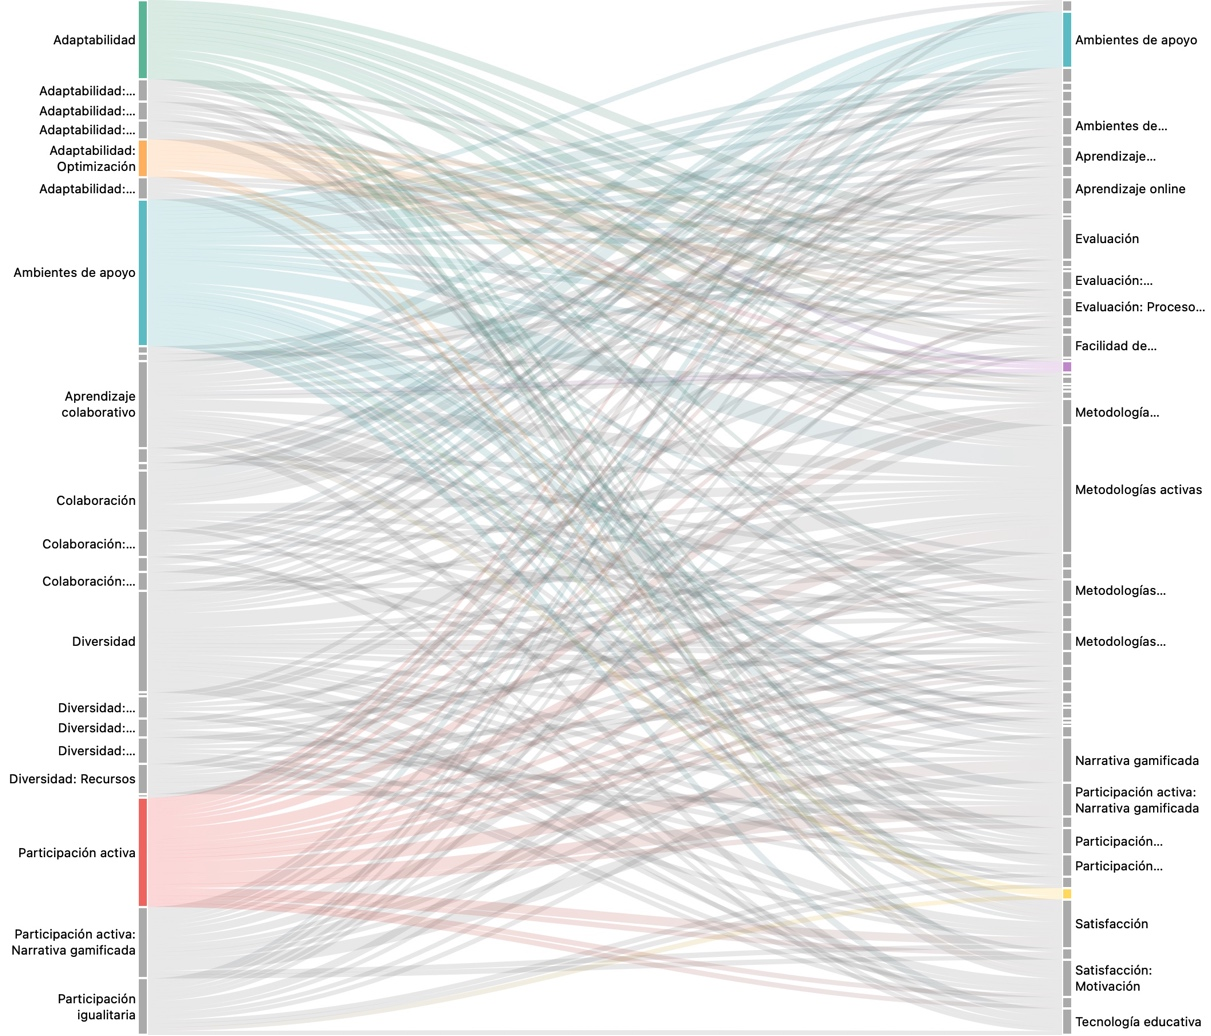
\includegraphics[width=\textwidth]{Imagem13.png}
\source{Elaboración propia.}
\end{minipage}
\end{figure}

\section{Considerações finais}\label{sec-consideraçõesfinais}

A partir da análise da vivência educacional descrita, visualizamos as interações propiciadas pelo novo \textit{ethos}, advindo do ciberespaço e da cultura digital, em especial, em contexto pandêmico, no qual as múltiplas semioses foram articuladas e propiciaram o exercício de consciência e agência dos alunos e dos professores.

Os participantes puderam olhar criticamente para as relações entre o eu, o outro e o meio ambiente em suas comunidades locais, problematizando questões socioambientais durante a pesquisa e o registro fotográfico, além de agir socialmente mediante a produção de vídeos e HQs que foram divulgados à comunidade em geral em eventos institucionais, bem como na internet.

Além disso, a técnica \textit{photovoice} aliada aos multiletramentos e à pedagogia psicodramática potencializou a mixagem de gêneros, mídias e linguagens, cara ao novo \textit{ethos} proveniente da cultura digital, na qual fontes, autorias e gêneros se articulam de forma rizomática.

Reconhecidos os limites deste texto e de todo trabalho educacional – que se estabelece na tênue linha educação-mercado –, esperamos que ele possa ajudar a pensar em alguns caminhos para o trabalho crítico com tecnologias digitais em sala de aula, de forma colaborativa e interdisciplinar e com foco em questões de linguagem.


\section{Agradecimentos}

Este trabalho foi realizado no âmbito do Centro de Inteligência
Artificial da Universidade de São Paulo (C4AI -
\url{http://c4ai.inova.usp.br/}), com o apoio da Fundação de Amparo à Pesquisa
do Estado de São Paulo (processo FAPESP \#2019/07665-4) e da IBM. Este
projeto também foi apoiado pelo Ministério da Ciência, Tecnologia e
Inovações, com recursos da Lei N. 8.248, de 23 de outubro de 1991, no
âmbito do PPI-Softex, coordenado pela Softex e publicado como Residência
em TIC 13, DOU 01245.010222/2022-44. Além disso, contou com o apoio
financeiro do Edital PRPPG-UFBA 010/2024 -- Programa de Apoio a Jovens
Professores(as)/Pesquisadores(as) 2024 -- e do Edital FAPESB/CNPq
004/2023 -- Programa Primeiros Projetos.



\printbibliography\label{sec-bib}
%conceptualization,datacuration,formalanalysis,funding,investigation,methodology,projadm,resources,software,supervision,validation,visualization,writing,review
\begin{contributors}[sec-contributors]
\authorcontribution{Jackson Wilke da Cruz Souza}[conceptualization,datacuration,formalanalysis,methodology,software,supervision,validation,writing,review]
\authorcontribution{Pedro Semcovici}[datacuration,software,writing,review]
\authorcontribution{Thiago Alexandre Salgueiro Pardo}[conceptualization,supervision,writing,review]
\end{contributors}
\end{document}
